\section{Synteza dźwięku fletu}

W literaturze można znaleźć wiele podejść do syntezy dźwięku instrumentów dętych drewnianych. Ich modele są przedstawione zazwyczaj za pomocą różniczkowych równań fizycznych lub w postaci falowodów cyfrowych. 
%klarnet: https://www.researchgate.net/publication/4333455_Representation_of_solo_clarinet_music_by_physical_modeling_synthesis
%gestures: https://www.researchgate.net/publication/5323798_Gesture_synthesis_basic_control_of_a_flute_physical_model
%slide-flute perry cook: https://quod.lib.umich.edu/cache//b/b/p/bbp2372.1992.072/bbp2372.1992.072.pdf#page=1;zoom=75
Przykładem takiej pracy naukowej jest artykuł na temat modelu fizycznego klarnetu, w którym autorzy opisują równaniami różniczkowymi poszczególne elementy instrumentu dętego drewnianego \cite{flute_klarnet}. Inna praca naukowa porusza temat kontroli modelu fletu, w którym autorzy skupili się na opisaniu zależnościach fizycznych związanych z grą flecisty \cite{flute_flecista}, takich jak: ciśnienie w ustach instumentalisty, odległość od fletu oraz szerokość otwarcia ust. Kolejnym przykładem artykułu opisującego model instrumentu dętego drewnianego jest praca P. Cooka przedstawiająca falowody cyfrowe fletu suwakowego (ang. slide flute) oraz klarnetu \cite{flute_cook}.

%o tym ze trudno jest zrobić wielootworowe --> ta ksiazka computer music costam


W niniejszym podrozdziale przedstawiono dwa podejścia do implementacji syntezy dźwięku drewnianego instrumentu dętego:
\begin{itemize}
	\setlength\itemsep{-3pt}
	\item za pomocą falowodu cyfrowego,
	\item za pomocą zidentyfikowanego modelu ARMA.
\end{itemize}
Na końcu podrozdziału przedstawiono wyniki porównujące oba te podejścia do syntezy na podstawie zsyntezowanych dźwięków.

\subsection{Synteza falowodowa dźwięku fletu}
%https://ccrma.stanford.edu/~jos/pasp/Digital_Waveguide_Models.html
%https://quod.lib.umich.edu/cache//b/b/p/bbp2372.1992.072/bbp2372.1992.072.pdf#page=1;zoom=75

Synteza falowodowa instrumentów dętych drewnianych opiera się głównie na cyfrowych liniach opóźniających, które symulują odbicia fali w komorze dźwiękowej (ang. bore) tego rodzaju instrumentów. Komorę dźwiękową można uprościć do cylindra, w którym rozchodzi się fala. Jest to znaczna zaleta metody falowodowej, gdyż dowolny element instrumentu może zostać zamodelowany za pomocą zestawu tub cylindrycznych.

\begin{equation} \label{equ:flute_row_falowe}
\frac{\partial^2 p}{\partial t^2} = \frac{\partial^2 p}{\partial x^2}
\end{equation}
\begin{tabular}{ l l l l}
	gdzie: 	&	$p$ & - &  ciśnienie, \\
	& $c$ &  - & prędkość propagacji dźwięku w powietrzu, \\
	&	$x$ & - &  długość korpusu instrumentu dętego,\\
	&	$t$ & - &  czas, \\
\end{tabular} \\

%https://sound.eti.pg.gda.pl/student/eim/synteza/macmal/
Powyższe jednowymiarowe równanie falowe przedstawia rozchodzenie się fali płaskiej w nieskończenie długim cylindrze. Rozwiązaniem równania (\ref{equ:flute_row_falowe}) jest superpozycja dwóch fal ciśnienia rozchodzących się w przeciwnych kierunkach komory dźwiękowej instrumentu dętego.


\subsubsection{Model}
W niniejszej pracy, syntezę falowodową dźwięku instrumentu dętego drewnianego oparto o schemat blokowy przedstawiony przez P. Cooka w 1992 roku.

\begin{figure}[H]
	\centering
	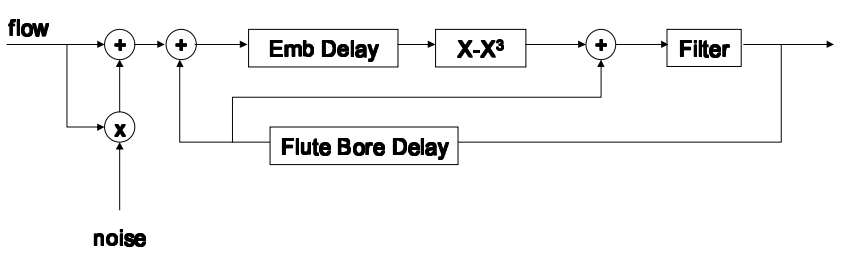
\includegraphics[width=14cm]{grafiki/flute_waveguide_mod}
	\captionsetup{justification=centering}
	\caption{Model falowodowy prostego instrumentu dętego drewnianego.}
	\label{rys:flute_cook}
\end{figure}

%https://courses.cs.washington.edu/courses/cse467/05wi/pdfs/lectures/15-waveguideInstruments.pdf
Wejściem systemu przedstawionego na rysunku \ref{rys:flute_cook} jest przepływ powietrza. Szum zostaje dodany w celu symulowania odgłosu wydechu flecisty. Interakcja między ustnikiem a komorą dźwiękową fletu przedstawiona została równaniem matematycznym $x-x^3$. Końcówka komory dźwiękowej fletu odbija niskie częstotliwości. Ta część schematu zostaje zasymulowana poprzez dodanie filtru dolnoprzepustowego. Obliczenie jednej próbki syntezowanego dźwieku na podstawie rysunku \ref{rys:flute_cook} wymaga 9 mnożeń oraz 6 operacji sumowania.

\subsubsection{Implementacja}
W autorskim programie realizowanym na procesorze DSP wzorowano się na schemacie \ref{rys:flute_cook}. Przepływ powietrza został zaimplementowany jako jedna sinusoida o odpowiedniej obwiedni \cite{flute_prezka}. Szum dochodzący do utworzonego sygnału został zasymulowany funkcją rand(), a jego ilość zostaje zeskalowana. 

... TODO ...

\subsection{Synteza dźwięku fletu na podstawie modelu ARMA}
W tym punkcie przedstawiono identyfikację modelu matematycznego fletu, na podstawie którego przeprowadzono później syntezę dźwięku. Do rozpoznania modelu instrumentu użyto tonu "A" razkreślnego o częstotliwości 440Hz. Dźwięk wygenerowany przez grę na flecie zmienia swoją charakterystykę w czasie. Oznacza to, iż jego model również zmienia się w trakcie nagranego przebiegu sygnału. Do identyfikacji wybrano te część nagrania dźwięku fletu, w której model instrumentu jest w stanie ustalonym.

\subsubsection{Identyfikacja modelu}
Identyfikacja modelu matematycznego instrumentu została przeprowadzona dwoma sposobami: 
\begin{itemize}
	\item poprzez manualne dopasowanie zer i biegunów modelu, 
	\item za pomocą funkcji wbudowanej w środowisko symulacyjne Matlab.
\end{itemize}

Proces identyfikacji przeprowadzono w środowisku symulacyjnym Matlab. Na nagranym fragmencie sygnału przeprowadzono dyskretną transformację Fouriera za pomocą algorytmu FFT.

% WYKRESSSSS
\begin{figure}[H]
	\centering
	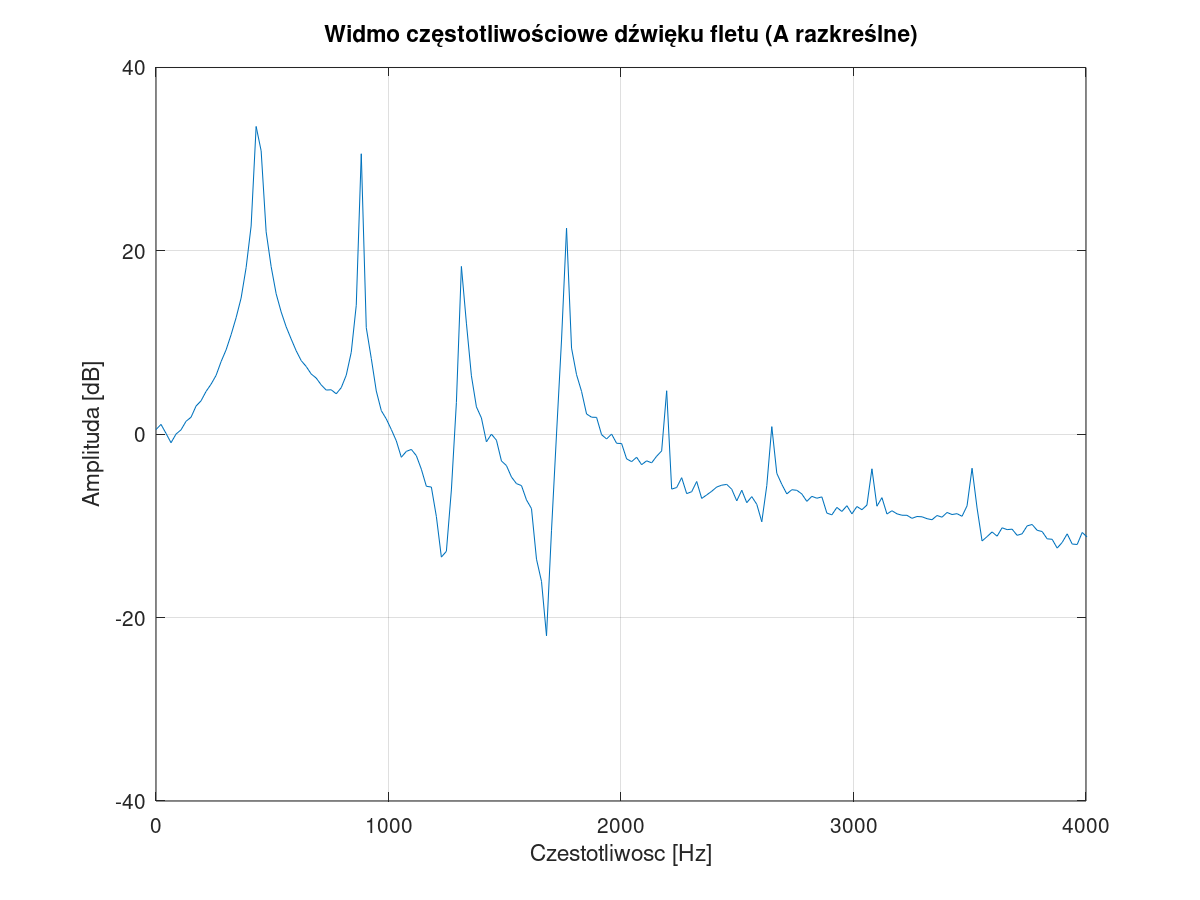
\includegraphics[width=12cm]{grafiki/flute_spectrum_orig}
	\captionsetup{justification=centering}
	\caption{Charakterystyka amplitudowa nagranego sygnału fletu.}
	\label{rys:flute_spectrum}
\end{figure}
% WYKRESSSS

Na rysunku \ref{rys:flute_spectrum} można zauważyć wyraźne piki oraz doliny charakterystyki częstotliwościowej nagranego sygnału. Siedem pierwszych pików charakterystyki zostało zinterpretowanych jako bieguny modelu, natomiast sześć pierwszych dolin zostały potraktowane jako jego zera. Liczba wybranych pików i dolin wziętych pod uwagę przy tworzeniu modelu, została dobrana na podstawie wzrokowej oceny ilości harmonicznych mogących mieć znaczny wpływ na ukształtowanie brzmienia zsyntezowanego instrumentu. Częstotliwości rezonansowe przetworzono według zależności:
\begin{equation} \label{equ:flute_bieguny}
p = 1-\frac{0.05}{A_{p}}e^{jf_{p}2\pi/F_{s}}
\end{equation}
\begin{equation} \label{equ:flute_doliny}
q = 1-\frac{0.05}{A_{q}}e^{jf_{q}2\pi/F_{s}}
\end{equation}
\begin{tabular}{ l l l l}
	gdzie: & $p$ &  - & bieguny modelu, \\
	&	$q$ & - &  zera modelu, \\
	&	$F_{s}$ & - &  częstotliwość próbkowania nagranego dźwięku,\\
	&	$f_{p,q}$ & - &  częstotliwość rezonansowa biegunów i zer modelu, \\
	&	$A_{p,q}$ & - &  amplituda rezonansu zer i biegunów, \\
\end{tabular} \\

Każdy pik charakterystyki został przetworzony na dwa bieguny odbite lustrzanie względem osi rzeczywistej na płaszczyźnie Z, według wzoru (\ref{equ:flute_bieguny}). Każda z dolin została odwzorowana jako dwa zera odbite lustrzanie względem osi Z, według wzoru (\ref{equ:flute_doliny}).

Model ARMA zsyntezowanego fletu utworzono na podstawie wyznaczonych zer i biegunów. W celu wygenerowania dźwięku z modelu w środowisku symulacyjnym, pobudzono go szumem białym. Następnie znormalizowano otrzymany sygnał, aby uniknąć przesterowań. Dźwięk wygenerowany z modelu przypomina brzmienie instrumentu z rodziny instrumentów dętych drewnianych. Wysokość wygenerowanego dźwięku jest taka sama jak w oryginalnym nagraniu (440Hz).

\subsubsection{Parametryzacja zidentyfikowanego modelu}
Gra na instrumencie wymaga wydobywania z niego dźwięków o różnej wysokości. Zidentyfikowany w poprzednim punkcie model jest statyczny - po pobudzeniu modelu szumem, wydobywa się z niego zawsze dźwięk o tej samej częstotliwości podstawowej ("A" razkreślny, na podstawie którego, model był identyfikowany). W celu wydobycia innego tonu na podstawie utworzonego modelu, należy dokonać jego parametryzacji. Parametryzacja zidentyfikowanego modelu polega na uzależnieniu każdego biegunu i zera modelu od pożądanego tonu.

Parametryzacja modelu opierać się będzie o zasady przyjęte w protokole MIDI. 
Na podstawie wzoru (\ref{equ:wpr_dzwiek}), każdy biegun został uzależniony od częstotliwości podstawowej zidentyfikowanego modelu. Częstotliwość podstawowa wymnożona przez pierwiastek dwunastego stopnia podniesiony do potęgi różnicy półtonów między częstotliwością 440Hz a częstotliwością pożądanego dźwięku pozwoliła utworzyć bieguny oraz zera w odpowiednim miejscu.
\begin{figure}[H]
	\centering
	\includegraphics[width=12cm]{grafiki/Model_B_A}
	\label{rys:por_mod_flet}
	\captionsetup{justification=centering}
	\caption{Porownanie modeli fletu dla dzwieku "B" razkreślnego (wykres przesuniety w prawo) i "A" razkreślnego (wykres przesunięty w lewo)}
	\label{rys:por_mod_flet}
\end{figure}
Na rysunku \ref{rys:por_mod_flet} widać, iż wszystkie piki oraz doliny opisane zidentyfikowanym modelem przesuwają się w dziedzinie częstotliwości dla różnych tonów. Oznacza to, iż pobudzony model wyda dźwięk o różnej wysokości dla różnych parametrów wejściowych.


\subsection{Synteza dźwięku fletu na podstawie zidentyfikowanego modelu AR oraz ARMA}
W tym podrozdziale zsyntezowany dźwięk zostanie wytworzony na podstawie modelu znalezionego w sposób algorytmiczny. Poszukiwane będą modele w postaci AR oraz ARMA dla dźwięku fletu, a następnie porównane pod względem rzędu oraz brzmienia po ich pobudzeniu.

W celu znalezienia modelu AR zaimplementowano estymator Yula-Walkera, który opiera się na wyliczeniu autokorelacji sygnału identyfikowanego procesu \cite{Y_W}. Rezultatem takiej estymacji są współczynniki procesu AR. Rząd modelu potrzebny do odnalezienia odpowiednio brzmiącego zsyntezowanego fletu wyniósł 300.

W celu znalezienia modelu autoregresyjnego ze średnią ruchomą użyto gotowej funkcji "armax()" wbudowanej w środowisko symulacyjne Matlab. Funkcja "armax()" pobiera dwa argumenty - sygnał, którego model jest identyfikowany oraz rząd mianownika i licznika tego modelu \cite{armax}. Estymator ten wykorzystuje zapętloną metodę przewidywania błędu do wykrywania parametrów modelu ARMA. Rząd modelu ARMA, który dawał dobre rezultaty po pobudzeniu go szumem (brzmiał podobnie do pierwotnego sygnału fletu) wyniósł 100. Przy takim rzędzie wciąż można usłyszeć 'cyfrowość' sygnału. Sygnał zsyntezowanego fletu brzmiał bardzo dobrze przy pobudzeniu modelu o rzędzie 500.

\begin{figure}[H]
	\centering
	\includegraphics[width=12cm, height=5cm]{grafiki/Model_AR_300}
	\captionsetup{justification=centering}
	\caption{Porownanie widm częstotliwości zidentyfikowanych modeli fletu w postaci AR oraz ARMA. Od lewej: Oryginalne widmo sygnału, widmo sygnału zidentyfikowanego procesu AR rzędu 300, widmo sygnału zidentyfikowanego procesu ARMA rzędu 100}
	\label{rys:por_ar_arma}
\end{figure}
Na rysunku \ref{rys:por_ar_arma} dokonano porównania widm częstotliwościowych dla różnych rzędów zidentyfikowanych modeli AR i ARMA. Wrażenia słuchowe są lepsze dla modelu ARMA 100 rzędu niż modelu AR 300 rzędu.

\subsubsection{Implementacja}

\subsection{Interfejs użytkownika}

\subsection{Wyniki}